\section*{Proposal}

Unmanned surface vehicles (USVs) are increasingly being used for maritime surveillance
to assist with law enforcement, military, and environmental monitoring.
Situational awareness is crucial for such USVs to operate safely and effectively,
and a big part of that is being able to detect and track waterlines.
Furthermore, approaching surface bodies usually appear in the waterline first,
so better waterline detection can help detect such objects earlier and
respond accordingly.
However, accurate waterline detection is difficult because of water reflections,
water surface glint, and cloud clutter~\cite{zhan-2017}.

\begin{figure}[h!]
  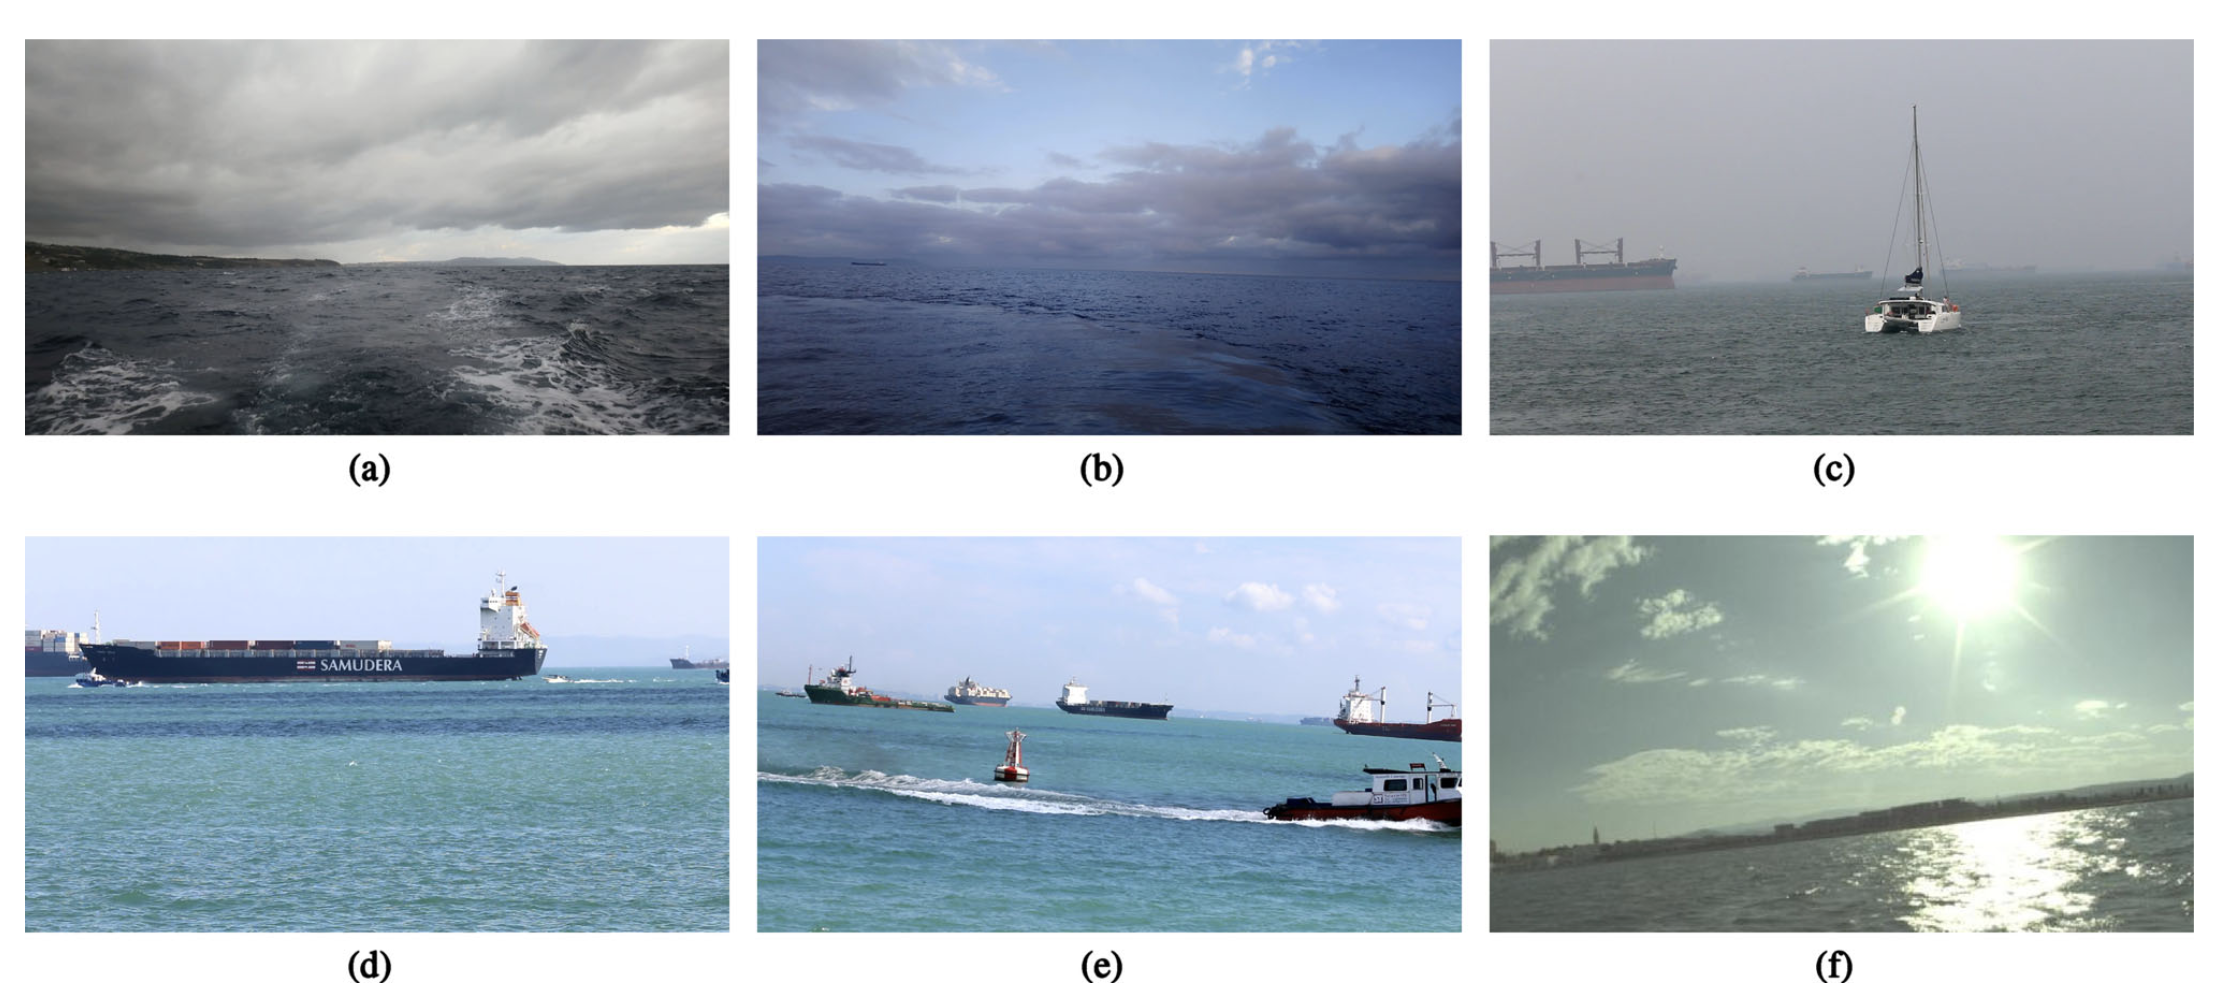
\includegraphics[width=\textwidth]{challenging-maritime-landscapes.png}
  \caption{
    Some of the main challenges faced in maritime waterline detection:
    \textbf{(a)} two classes above the horizon,
    \textbf{(b)} low contrast,
    \textbf{(c)} low contrast due to fog,
    \textbf{(d)} horizon occlusion and prominent ship lines,
    \textbf{(e)} horizon occlusion and a prominent wake line,
    \textbf{(f)} dark coast and strong sun reflection on the sea surface
    \cite{zardoua-2021}.
  }
\end{figure}
Various techniques have been proposed to detect waterlines,
including use of Hough transforms to detect edges and predict which edge
is most likely to be the waterline~\cite{gao-2007} and \cite{prasad-2017},
use of gradient maps to identify candidate points, which are then constrained
to a line by the \textsc{RANSAC} algorithm~\cite{zhan-2017},
and the use of semantic segmentation with CNNs to isolate regions~\cite{bovcon-2020}.
These methods face several challenges ---
the Hough transform method and the \textsc{RANSAC} method are sensitive to noise
and difficult difficult to use for non-linear waterlines,
while the segmentation method needs to identify and isolate
\emph{every} object in its view, resulting in computational redundancies
and difficulty in identifying the waterline when new objects that the CNN
has not encountered before are in the view~\cite{bovcon-2020}.

\step
This research project seeks to develop more robust techniques for
waterline detection in USVs. Improvements in waterline detection will
improve state estimation and obstacle detection, since USVs will be able to
focus on the most-important parts of their view.
